\documentclass[a4paper]{article}
\usepackage[a4paper,margin=0mm]{geometry}
\usepackage{fontspec}
\usepackage{unicode-math}
\usepackage{amsmath}
\usepackage{tikz}
\usepackage[table]{xcolor}
\usepackage[absolute]{textpos}
\usepackage{enumitem}
\usepackage{array}
\usepackage{multirow}

\setmainfont{Libertinus Serif}
\setsansfont{Libertinus Sans}
\setmathfont{Libertinus Math}
\newfontfamily\trackedsans{Libertinus Sans}[LetterSpace=8.0]

\definecolor{accent}{HTML}{F46530}
\definecolor{badge}{HTML}{FFBDA5}
\definecolor{ink}{HTML}{2A2E30}

\setlength{\TPHorizModule}{1mm}
\setlength{\TPVertModule}{1mm}
\setlength{\parindent}{0pt}
\pagestyle{empty}

\newcommand{\LCOL}{16mm}
\newcommand{\RCOL}{111mm}
\newcommand{\COLW}{83mm}

\newcommand{\topicheader}[2]{%
\begin{textblock*}{194mm}(16mm,10mm)
\begin{tikzpicture}
\node[fill=accent,text=white,font=\sffamily\bfseries\fontsize{13}{13}\selectfont,
      minimum width=9mm,minimum height=9mm,inner sep=0pt] at (4.5mm,-4.5mm) {#1};
\node[font=\sffamily\bfseries\fontsize{15}{16}\selectfont,text=ink,anchor=west] at (12mm,-4.5mm) {#2};
\end{tikzpicture}
\end{textblock*}
\begin{textblock*}{194mm}(16mm,22.5mm)

\begin{tikzpicture}
\fill[accent] (0,0) rectangle (194mm,0.5mm);
\end{tikzpicture}
\end{textblock*}
}

\newcommand{\pagefooter}[1]{%
\begin{textblock*}{194mm}(8mm,286.41mm)
  
\begin{tikzpicture}
    \fill[accent] (0,0) rectangle (194mm,0.6mm);
  \end{tikzpicture}
\end{textblock*}
\begin{textblock*}{63.59mm}(8mm,288.27mm)
  {\sffamily\bfseries\color{accent}\fontsize{13}{16}\selectfont SAT 1200+}
\end{textblock*}
\begin{textblock*}{10mm}(188mm,288.27mm)
  \centering{\sffamily\color{accent}\fontsize{14}{16}\selectfont #1}
\end{textblock*}
}

\newcommand{\colrule}[2]{%
\begin{textblock*}{1mm}(105mm,#1mm)
\begin{tikzpicture}
\draw[black!65,line width=0.5pt] (0,0) -- (0,#2mm);
\end{tikzpicture}
\end{textblock*}
}

\newcommand{\setkicker}[2]{%
{\sffamily\bfseries\fontsize{12}{14}\selectfont #1.}\ {\itshape\fontsize{11}{14}\selectfont\color{black!75} #2}\par\vspace{2mm}%
}

\setlength{\fboxsep}{1.4pt}
\setlength{\fboxrule}{0.5pt}
\newcommand{\pnum}[1]{\fcolorbox{ink}{white}{\sffamily\bfseries\fontsize{8}{8}\selectfont #1}~}

\newcommand{\qrbox}[1]{%
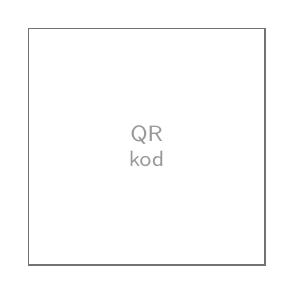
\begin{tikzpicture}
\draw[black!55,line width=0.6pt] (0,0) rectangle (30mm,30mm);
\node[black!40,font=\sffamily\fontsize{8}{9}\selectfont,align=center] at (15mm,15mm) {QR\\kod};
\end{tikzpicture}\\[1.5mm]
{\sffamily\fontsize{9}{11}\selectfont\color{black!70} #1}%
}

\arrayrulecolor{accent}
\setlength{\arrayrulewidth}{0.7pt}
\renewcommand{\arraystretch}{1.35}
\newcommand{\anstitle}[1]{{\sffamily\bfseries\color{accent}\fontsize{11}{13}\selectfont #1}\\[1.3mm]}

\begin{document}

% ================= PAGE 1: Set 1 | Set 2 =================
\topicheader{2}{KASRLAR}
\pagefooter{1}
\colrule{32}{238}
\mbox{}%

\begin{textblock*}{\COLW}(\LCOL,32mm)
{\fontsize{12}{15}\selectfont
\setkicker{1-to'plam}{Qisqartiring -- javobni eng sodda ko'rinishda yozing.}

\noindent\pnum{1} $\dfrac{8}{12}=$\\[18mm]
\noindent\pnum{2} $\dfrac{15}{25}=$\\[18mm]
\noindent\pnum{3} $\dfrac{18}{24}=$\\[18mm]
\noindent\pnum{4} $\dfrac{21}{14}=$\\[18mm]
\noindent\pnum{5} $\dfrac{36}{48}=$\\[18mm]
\noindent\pnum{6} $\dfrac{50}{75}=$\\[18mm]
\noindent\pnum{7} $\dfrac{28}{35}=$\\[18mm]
\noindent\pnum{8} $\dfrac{100}{40}=$
}
\end{textblock*}

\begin{textblock*}{\COLW}(\RCOL,32mm)
{\fontsize{12}{15}\selectfont
\setkicker{2-to'plam}{Qo'shing yoki ayiring -- avval umumiy maxraj toping.}

\noindent\pnum{1} $\dfrac{1}{3}+\dfrac{1}{4}=$\\[18mm]
\noindent\pnum{2} $\dfrac{2}{5}+\dfrac{1}{3}=$\\[18mm]
\noindent\pnum{3} $\dfrac{3}{4}-\dfrac{1}{6}=$\\[18mm]
\noindent\pnum{4} $\dfrac{5}{6}-\dfrac{2}{9}=$\\[18mm]
\noindent\pnum{5} $\dfrac{1}{2}+\dfrac{2}{3}-\dfrac{1}{4}=$\\[18mm]
\noindent\pnum{6} $\dfrac{7}{10}-\dfrac{1}{4}=$\\[18mm]
\noindent\pnum{7} $\dfrac{3}{8}+\dfrac{5}{12}=$\\[18mm]
\noindent\pnum{8} $\dfrac{11}{12}-\dfrac{3}{4}=$
}
\end{textblock*}

\clearpage

% ================= PAGE 2: Set 3 | Set 4 =================
\topicheader{2}{KASRLAR}
\pagefooter{2}
\colrule{32}{238}
\mbox{}%

\begin{textblock*}{\COLW}(\LCOL,32mm)
{\fontsize{12}{15}\selectfont
\setkicker{3-to'plam}{Ko'paytiring -- hisoblashdan oldin qisqartirishga harakat qiling.}

\noindent\pnum{1} $\dfrac{2}{3}\times\dfrac{3}{5}=$\\[18mm]
\noindent\pnum{2} $\dfrac{4}{7}\times\dfrac{7}{8}=$\\[18mm]
\noindent\pnum{3} $\dfrac{5}{6}\times\dfrac{2}{3}=$\\[18mm]
\noindent\pnum{4} $\dfrac{3}{4}\times\dfrac{8}{9}=$\\[18mm]
\noindent\pnum{5} $\dfrac{7}{10}\times\dfrac{5}{14}=$\\[18mm]
\noindent\pnum{6} $\dfrac{2}{9}\times\dfrac{3}{4}=$\\[18mm]
\noindent\pnum{7} $\dfrac{5}{8}\times\dfrac{4}{15}=$\\[18mm]
\noindent\pnum{8} $\dfrac{9}{10}\times\dfrac{5}{6}=$
}
\end{textblock*}

\begin{textblock*}{\COLW}(\RCOL,32mm)
{\fontsize{12}{15}\selectfont
\setkicker{4-to'plam}{Bo'ling -- ikkinchi kasrni teskarisiga aylantirib ko'paytiring.}

\noindent\pnum{1} $\dfrac{2}{3}\div\dfrac{4}{5}=$\\[18mm]
\noindent\pnum{2} $\dfrac{3}{4}\div\dfrac{1}{2}=$\\[18mm]
\noindent\pnum{3} $\dfrac{5}{6}\div\dfrac{5}{9}=$\\[18mm]
\noindent\pnum{4} $\dfrac{7}{8}\div\dfrac{7}{4}=$\\[18mm]
\noindent\pnum{5} $\dfrac{2}{5}\div\dfrac{3}{10}=$\\[18mm]
\noindent\pnum{6} $\dfrac{9}{10}\div\dfrac{3}{5}=$\\[18mm]
\noindent\pnum{7} $\dfrac{4}{9}\div\dfrac{8}{3}=$\\[18mm]
\noindent\pnum{8} $\dfrac{5}{12}\div\dfrac{5}{6}=$
}
\end{textblock*}

\clearpage

% ================= PAGE 3: Set 5 | Set 6 (spot the error) =================
\topicheader{2}{KASRLAR}
\pagefooter{3}
\colrule{32}{238}
\mbox{}%

\begin{textblock*}{\COLW}(\LCOL,32mm)
{\fontsize{11.5}{14.5}\selectfont
\setkicker{5-to'plam}{Aralash son $\leftrightarrow$ noto'g'ri kasr.}

\noindent\pnum{1} $2\tfrac{3}{4}$ ni noto'g'ri kasrga aylantiring.\\[11mm]
\noindent\pnum{2} $5\tfrac{1}{6}$ ni noto'g'ri kasrga aylantiring.\\[11mm]
\noindent\pnum{3} $\dfrac{17}{5}$ ni aralash songa aylantiring.\\[11mm]
\noindent\pnum{4} $\dfrac{29}{4}$ ni aralash songa aylantiring.\\[11mm]
\noindent\pnum{5} $1\tfrac{1}{2}+2\tfrac{1}{3}=$ (aralash son)\\[11mm]
\noindent\pnum{6} $3\tfrac{1}{4}-1\tfrac{3}{4}=$ (aralash son)\\[11mm]
\noindent\pnum{7} $2\tfrac{2}{5}\times1\tfrac{1}{4}=$\\[11mm]
\noindent\pnum{8} $\dfrac{53}{6}$ ni aralash songa aylantiring.
}
\end{textblock*}

\begin{textblock*}{\COLW}(\RCOL,32mm)
{\fontsize{11}{14}\selectfont
\setkicker{6-to'plam}{Xatoni toping -- buzilgan qadamni ayting, to'g'ri javobni bering.}

\noindent\pnum{1} $\dfrac{1}{3}+\dfrac{1}{4}$ ifodasida ko'rsatilgan yechimda xato bor:\\[1mm]
\hspace*{7mm}\textit{``$\dfrac{1+1}{3+4}=\dfrac{2}{7}$.''}\\[2mm]
\hspace*{7mm}Xato va to'g'ri javob: \makebox[52mm]{\dotfill}\\[8mm]

\noindent\pnum{2} $\dfrac{2}{5}+\dfrac{2}{5}$ ifodasida ko'rsatilgan yechimda xato bor:\\[1mm]
\hspace*{7mm}\textit{``Suratni saqlab, maxrajlarni qo'shamiz: $\dfrac{2}{10}$.''}\\[2mm]
\hspace*{7mm}Xato va to'g'ri javob: \makebox[52mm]{\dotfill}\\[8mm]

\noindent\pnum{3} $\dfrac{3}{4}\div\dfrac{2}{5}$ ifodasida ko'rsatilgan yechimda xato bor:\\[1mm]
\hspace*{7mm}\textit{``$\dfrac{4}{3}\times\dfrac{2}{5}=\dfrac{8}{15}$.''}\\[2mm]
\hspace*{7mm}Xato va to'g'ri javob: \makebox[52mm]{\dotfill}\\[8mm]

\noindent\pnum{4} $\dfrac{16}{24}$ ni soddalashtirishda ko'rsatilgan yechimda xato bor:\\[1mm]
\hspace*{7mm}\textit{``2 ga qisqartirib, $\dfrac{8}{12}$ -- tayyor.''}\\[2mm]
\hspace*{7mm}Xato va to'g'ri javob: \makebox[52mm]{\dotfill}\\[8mm]

\noindent\pnum{5} $2\tfrac{3}{4}$ ni noto'g'ri kasrga aylantirishda ko'rsatilgan yechimda xato bor:\\[1mm]
\hspace*{7mm}\textit{``$\dfrac{2+3}{4}=\dfrac{5}{4}$.''}\\[2mm]
\hspace*{7mm}Xato va to'g'ri javob: \makebox[52mm]{\dotfill}
}
\end{textblock*}

\clearpage

% ================= PAGE 4: Set 7 (bonus) =================
\topicheader{2}{KASRLAR}
\pagefooter{4}
\colrule{32}{238}
\mbox{}%

\begin{textblock*}{\COLW}(\LCOL,32mm)
{\fontsize{12}{15}\selectfont
\setkicker{7-to'plam}{Bonus / qiyin -- har biriga taxminan 90 soniya.}

\noindent\pnum{1} $\left(\dfrac{1}{2}+\dfrac{1}{3}\right)\times\dfrac{2}{5}=$\\[26mm]
\noindent\pnum{2} $3\tfrac{1}{2}\div\left(\dfrac{1}{4}+\dfrac{1}{4}\right)=$\\[26mm]
\noindent\pnum{3} $\left(\dfrac{2}{3}-\dfrac{1}{6}\right)\times\left(\dfrac{3}{4}+\dfrac{1}{2}\right)=$\\[26mm]
\noindent\pnum{4} $1\tfrac{3}{4}\times\dfrac{2}{7}+\dfrac{1}{8}=$\\[26mm]
\noindent\pnum{5} $\left(\dfrac{5}{6}\div\dfrac{5}{9}\right)-\left(\dfrac{1}{2}\times\dfrac{2}{3}\right)=$
}
\end{textblock*}

\clearpage

% ================= PAGE 5: Javoblar -- unified answer table =================
\topicheader{2}{KASRLAR}
\pagefooter{5}
\mbox{}%

\begin{textblock*}{194mm}(16mm,30mm)
{\bfseries\itshape\color{accent}\fontsize{19}{21}\selectfont\centering Javoblar\par}
\end{textblock*}

\begin{textblock*}{194mm}(16mm,38mm)
{\fontsize{9.3}{11.5}\selectfont
\centering
\renewcommand{\arraystretch}{1.3}
\begin{tabular}{|>{\centering\arraybackslash}p{26mm}|>{\centering\arraybackslash}p{10mm}|>{\centering\arraybackslash}p{28mm}|>{\centering\arraybackslash}p{10mm}|>{\centering\arraybackslash}p{28mm}|}
\hline
\rowcolor{badge!55}\textbf{To'plam} & \textbf{\#} & \textbf{Javob} & \textbf{\#} & \textbf{Javob}\\
\hline
\multirow{4}{26mm}{\centering 1-to'plam} & 1 & $\frac{2}{3}$ & 2 & $\frac{3}{5}$\\\cline{2-5}
 & 3 & $\frac{3}{4}$ & 4 & $\frac{3}{2}$\\\cline{2-5}
 & 5 & $\frac{3}{4}$ & 6 & $\frac{2}{3}$\\\cline{2-5}
 & 7 & $\frac{4}{5}$ & 8 & $\frac{5}{2}$\\\hline
\multirow{4}{26mm}{\centering 2-to'plam} & 1 & $\frac{7}{12}$ & 2 & $\frac{11}{15}$\\\cline{2-5}
 & 3 & $\frac{7}{12}$ & 4 & $\frac{11}{18}$\\\cline{2-5}
 & 5 & $\frac{11}{12}$ & 6 & $\frac{9}{20}$\\\cline{2-5}
 & 7 & $\frac{19}{24}$ & 8 & $\frac{1}{6}$\\\hline
\multirow{4}{26mm}{\centering 3-to'plam} & 1 & $\frac{2}{5}$ & 2 & $\frac{1}{2}$\\\cline{2-5}
 & 3 & $\frac{5}{9}$ & 4 & $\frac{2}{3}$\\\cline{2-5}
 & 5 & $\frac{1}{4}$ & 6 & $\frac{1}{6}$\\\cline{2-5}
 & 7 & $\frac{1}{6}$ & 8 & $\frac{3}{4}$\\\hline
\multirow{4}{26mm}{\centering 4-to'plam} & 1 & $\frac{5}{6}$ & 2 & $\frac{3}{2}$\\\cline{2-5}
 & 3 & $\frac{3}{2}$ & 4 & $\frac{1}{2}$\\\cline{2-5}
 & 5 & $\frac{4}{3}$ & 6 & $\frac{3}{2}$\\\cline{2-5}
 & 7 & $\frac{1}{6}$ & 8 & $\frac{1}{2}$\\\hline
\multirow{4}{26mm}{\centering 5-to'plam} & 1 & $\frac{11}{4}$ & 2 & $\frac{31}{6}$\\\cline{2-5}
 & 3 & $3\frac{2}{5}$ & 4 & $7\frac{1}{4}$\\\cline{2-5}
 & 5 & $3\frac{5}{6}$ & 6 & $1\frac{1}{2}$\\\cline{2-5}
 & 7 & $3$ & 8 & $8\frac{5}{6}$\\\hline
\multirow{3}{26mm}{\centering 7-to'plam} & 1 & $\frac{1}{3}$ & 2 & $7$\\\cline{2-5}
 & 3 & $\frac{5}{8}$ & 4 & $\frac{5}{8}$\\\cline{2-5}
 & 5 & $\frac{7}{6}$ & -- & --\\\hline
\multirow{5}{26mm}{\centering 6-to'plam} & \multicolumn{4}{p{76mm}|}{1.\ Surat/maxraj mustaqil qo'shilgan, umumiy maxraj topilmagan. To'g'ri: $\frac{1}{3}=\frac{4}{12}$, $\frac{1}{4}=\frac{3}{12}$, yig'indi $\frac{7}{12}$.}\\\cline{2-5}
 & \multicolumn{4}{p{76mm}|}{2.\ Maxrajlar teng bo'lsa, faqat suratlar qo'shiladi. To'g'ri: $\frac{2}{5}+\frac{2}{5}=\frac{4}{5}$.}\\\cline{2-5}
 & \multicolumn{4}{p{76mm}|}{3.\ Teskari kasr ikkinchi (bo'luvchi) kasrga qo'llanishi kerak edi. To'g'ri: $\frac{3}{4}\times\frac{5}{2}=\frac{15}{8}$.}\\\cline{2-5}
 & \multicolumn{4}{p{76mm}|}{4.\ Bitta qisqartirishdan keyin to'xtagan (8 va 12 hali 4 ga bo'linadi). To'g'ri: $\frac{16}{24}=\frac{2}{3}$.}\\\cline{2-5}
 & \multicolumn{4}{p{76mm}|}{5.\ Butun son maxrajga ko'paytirilmagan. To'g'ri: $3\times4=12$, $12+3=15$, ya'ni $\frac{11}{4}$.}\\\hline
\end{tabular}
}
\end{textblock*}

\begin{textblock*}{194mm}(16mm,228mm)
\centering
{\sffamily\fontsize{9.5}{11.5}\selectfont\color{black!70} Video yechimlar va qo'shimcha testlar uchun quyidagi QR kodlarni skanerlang:}\\[4mm]
\begin{minipage}[t]{32mm}\centering\qrbox{YouTube}\end{minipage}%
\hspace{16mm}%
\begin{minipage}[t]{32mm}\centering\qrbox{Telegram}\end{minipage}
\end{textblock*}

\end{document}
